% Tento soubor nahraďte vlastním souborem s obsahem práce.
%=========================================================================
% Autoři: Michal Bidlo, Bohuslav Křena, Jaroslav Dytrych, Petr Veigend a Adam Herout 2019

% Pro kompilaci po částech (viz projekt.tex), nutno odkomentovat a upravit
%\documentclass[../projekt.tex]{subfiles}
%\begin{document}

\chapter{Úvod}
%cca strana

\chapter{Použitý Hardware}
Celá práce je implementována nad existujícím hardwarem. Konkrétně se jedná o stavebnici Adeept AWR 4WD. Její součástí jsou všechny použité motory, serva, čidla a další periferie. Mozkem, na kterém poběží software zajišťující ovládání těchto komponent, bude mikropočítač Raspberry Pi 4.

\section{HW Technologie}
Nejprve budou představeny obecné hardwarové technologie které jsou následně využívány některými z představovaných periferií.

\subsection*{Pulzně šířková modulace}
Jedná se o techniku, která umožňuje vytvořit pseudo-analogový výstup s použitím číslicových výstupů. Mikrokontroléry jsou digitální zařízení a chtěly by tedy s okolním světem komunikovat pomocí jedniček a nul. Reálný svět tak ovšem nefunguje a proto je často potřeba převádět výstup z mikrokontroléru na analogový signál. Problém je v tom, že převod digitálního signálu na analogový je relativně dlouhá a neefektivní operace. Proto vznikla pulzně šířková modulace (PWM), která umožňuje relativně jednoduše simulovat analogový výstup. \cite{embeded_robotics}

PWM využívá toho, že člověk nedokáže rozpoznat rychlé změny, například led dioda blikající na frekvenci 5000 Hz se člověku jeví jako by svítila permanentně. Mechanická zařízení také mívají relativně velkou latenci a dc motoru tedy nevadí, že místo konstantního analogového napětí dostává periodický číslicový signál. \cite{embeded_robotics}

\begin{figure}[h!]
	\centering
	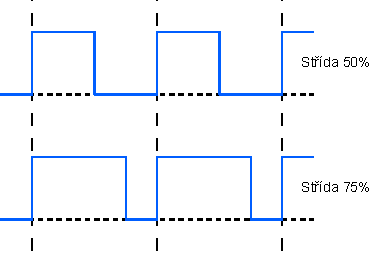
\includegraphics[scale=1]{obrazky-figures/pwm_duty_cycle.pdf}
	\caption{PWM signál pro různé hodnoty střídy}
	\label{}
\end{figure}

Při pohledu na klasický digitální signál který rovnoměrně střídá vysokou a nízkou úroveň by šlo říci, že se jedná o PWM signál se střídou 50\%. Střída (duty cycle) udává poměr času, kdy je signál v logické jedničce, ku času, kdy je v nule. Součet těchto hodnot se musí rovnat délce jedné periody. Úpravou tohoto poměru lze simulovat analogový signál. \cite{embeded_robotics}

\subsection*{I2C}
Je synchronní sběrnice, která se vyznačuje svou jednoduchostí a nízkou cenou. Využívá dva vodiče SDA (serial data) a SCL (serial clock). Oba vodiče jsou připojeny k napájecímu napětí pomocí pull-up rezistoru a bez vlivu jiného hardwaru tedy zůstávají v logické jedničce. Zařízení, která jsou na tuto sběrnici připojeny, využívají open drain k úpravě aktuální napěťové úrovně. I2C pracuje s dvěma druhy zařízení, master a slave. Master zahajuje, řídí a ukončuje komunikaci na vodiči SDA a po dobu průběhu komunikace generuje hodinový signál na SCL. Typicky se jedná o mikrokontroler. Slave jsou pak ostatní zařízení s nimiž může master komunikovat, typicky různé periferie. \cite{embeded_robotics}

\begin{figure}[h!]
	\centering
	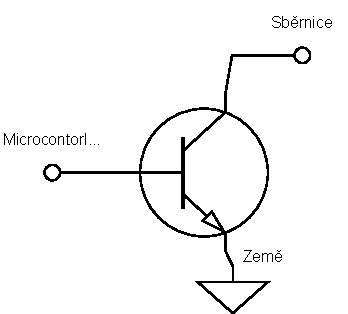
\includegraphics[scale=1]{obrazky-figures/open_drain.pdf}
	\caption{Open drain}
	\label{}
\end{figure}

Přenos jednoho datového rámce zahájí master zařízení přivedením datové sběrnice do nuly. Následující komunikace se skládá z odeslání rámce o délce osmi bitů a potvrzení o úspěšném přenosu dat od přijímajícího zařízení. Toto potvrzení se nazývá ACK a je provedeno podržením datové sběrnice v hodnotě nula po dobu jednoho taktu. Opačný stav se nazývá NACK a indikuje že nastala chyba. Ukončení přenosu je provedeno navrácením datové sběrnice na hodnotu jedna. \cite{um10204}

\begin{figure}[h!]
	\centering
	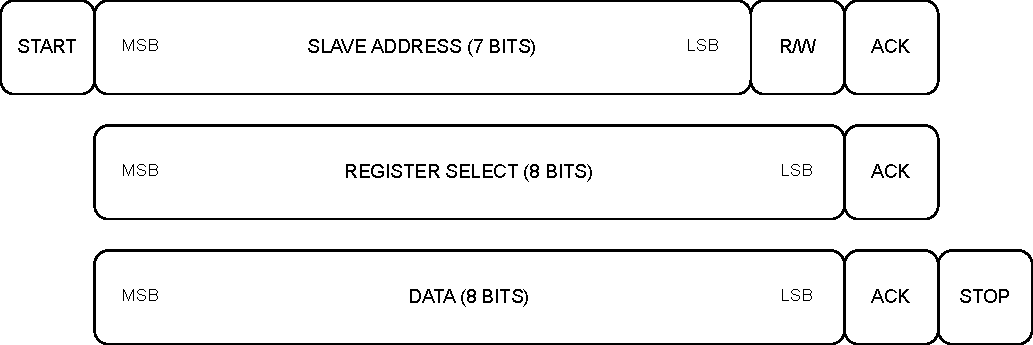
\includegraphics[scale=0.75]{obrazky-figures/i2c_data_word.pdf}
	\caption{Datové slovo sběrnice I2C}
	\label{}
\end{figure}

Na obrázku lze vidět, jak může vypadat přenos jednoho datového slova. V prvním rámci je přenesena sedmi bitová adresa, identifikující slave zařízení se kterým chce máster navázat komunikaci. Osmý bit datového rámce indikuje směr, kterým budou posílány data. V druhém rámci dojde k adresaci konkrétního registru na slave zařízení. A ve třetím, případně dalších, již probíhá samotné posílání dat mezi zařízeními. \cite{an4481}

\section{Adeept AWR 4WD}
Pohyb tohoto robota zajišťují čtyři pevná kola a zatáčení je tedy realizováno diferenciálním způsobem. To znamená, že jednotlivá kola se mohou otáčet svou vlastní rychlostí a zpomalením kol na jedné straně oproti té druhé lze provést zatáčení robota. Velkou výhodou tohoto přístupu je možnost otáčení robota na místě. Nevýhodou pak budou složitější výpočty při potřebě zahnout o nějaký přesně daný úhel.

\noindent Následující stránky popisují jednotlivé komponenty tohoto robota.

\subsection*{Robot HAT}
HAT(hardware attached on top) je hardwarová deska, která slouží k rozšíření mikrokontroléru o další funkcionalitu. Tato konkrétní se k Raspberyy Pi připojuje pomocí GPIO(General purpuse input outpu) pinů. Deska jako taková obsahuje rozšiřující čipy a rozhraní sloužící k ovládání připojených periferií.

\begin{itemize}
	\item{PCA9685 \cite{pca9685}}
	\begin{itemize}
		\item{generátor PWM signálu}
		\item{16 kanálů}
		\item{12 bitů rozlišení střídy (4096 možných hodnot)}
		\item{je ovládaný přes I2C sběrnici}
	\end{itemize}
	\item{L298P \cite{l298}}
	\begin{itemize}
		\item{ovladač pro řízení dc motoru}
		\item{základem je full bridge obvod}
		\item{umožňuje roztočit motor oběma směry}
		\item{pomocí PWM lze ovládat rychlost motorů}
		\item{připojuje motor na externí napájení}
	\end{itemize}
	\item{další rozhraní pro připojení periferií (sledování čáry, ultrazvukový senzor, led)}
\end{itemize}

\begin{figure}[h!]
	\centering
	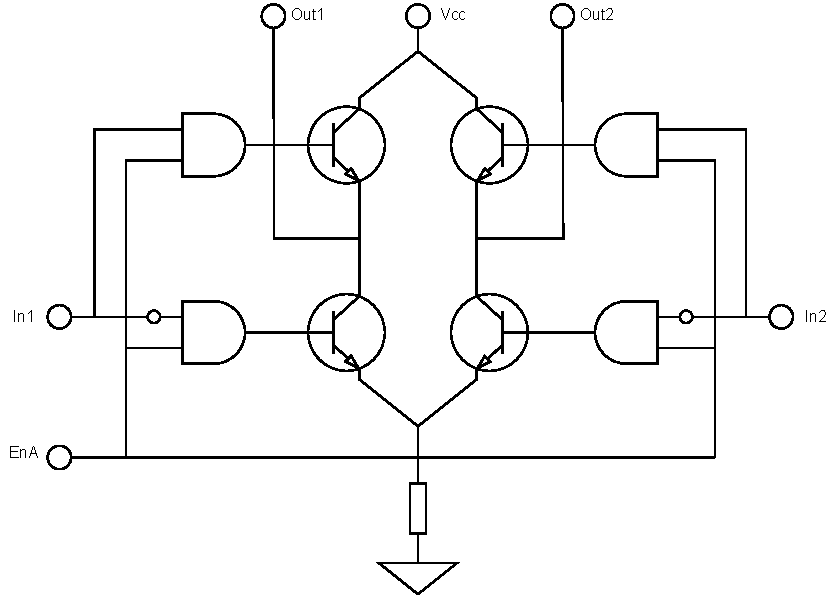
\includegraphics[scale=0.75]{obrazky-figures/motor_full_bridge.pdf}
	\caption[Full bridge ovladač motoru.]{Full bridge konfigurace pro ovládání motoru. In1 a In2 určují směr otáčení. EnA je PWM signál určující rychlost otáčení. \cite{l298}}
	\label{}
\end{figure}

\newpage
\subsection*{DC Motor}
Pohyb celého autíčka zajišťují čtyři stejnosměrným proudem(direct current) napájené motory. Ovladač motorů L298P je umístěný na Robot HAT.

\begin{figure}[h!]
	\centering
	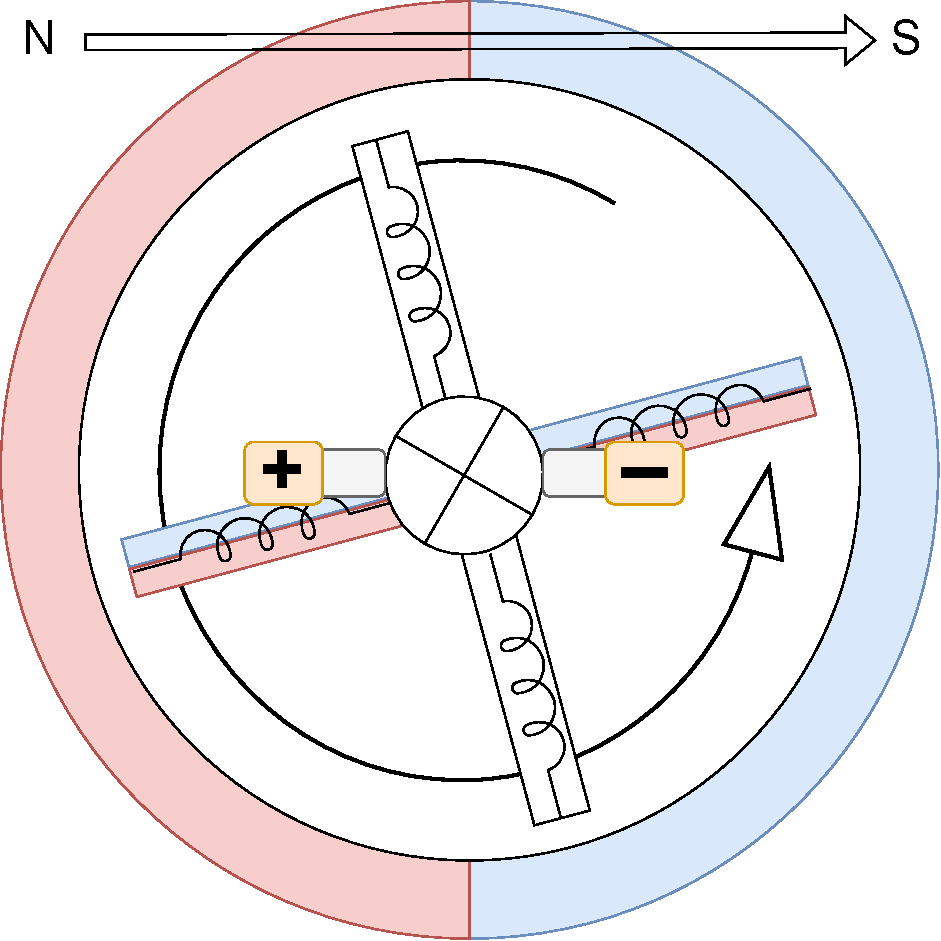
\includegraphics[scale=0.50]{obrazky-figures/dc_motor.pdf}
	\caption{Schéma DC motoru}
	\label{}
\end{figure}

Elektrický DC motor se skládá ze dvou hlavních částí, stator a rotor. Stator je statická, vnější část, a typicky se jedná o permanentní magnet. Uvnitř statoru se pak nachází rotor, ten se skládá z elektromagnetů, které při zapnutí reagují se statorem(opačné póly se přitahují a stejné odpuzují) a dojde tak k částečnému pootočení. Při správném spínání a vypínání těchto elektromagnetů lze motor rozběhnout. 
Toto střídání zajišťuje prstenec zvaný komutátor. Komutátor je rozdělen na několik od sebe odizolovaných částí, ke kterým jsou připojeny vývody elektromagnetů. S povrchem prstence jsou pomocí pružin v kontaktu dva kartáče. Tyto kartáče se již neotáčí a mohou tak být připojeny na zdroj napájení a zem. Komutátor se otáčí společně s rotorem a při tomto pohybu se kartáče postupně dotýkají různých částí komutátoru a spínají tak jednotlivé elektromagnety, ty zajistí pootočení rotoru a sepnutí následujícího magnetu. \cite{dc_motor}

\subsection*{Servo}
Servo je komponenta na první pohled podobná DC Motoru. Na rozdíl od něj se však neotáčí celých 360 stupňů, ale bývá omezena na nějakou menší hodnotu, například 180 stupňů. Hlavním výhodou a důvodem pro použití serva je plná kontrola nad úhlem natočení jeho hřídele. \cite{embeded_robotics}

\begin{figure}[h!]
	\centering
	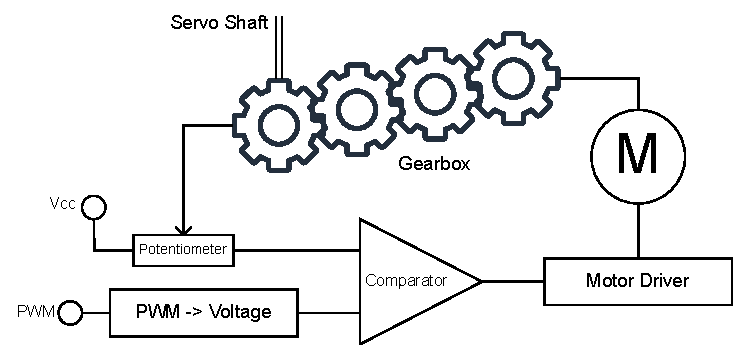
\includegraphics[scale=0.9]{obrazky-figures/servo.pdf}
	\caption{Vnitřní zapojení serva}
	\label{}
\end{figure}

Při pohledu na vnitřní zapojení serva lze zjistit, že se prakticky jedná o klasický dc motor připojený na převodovku a rozšířený o elektroniku na jeho řízení. K nastavení úhlu serva se využívá PWM signál. Ten je první přeložený na napěťovou úroveň, která je porovnána s aktuálním natočením serva a výsledek udává směr, kterým se bude otáčet motor. Aktuální natočení serva je získáno využitím potenciometru zapojeného na výstupní hřídel serva. \cite{embeded_robotics}

Adeept AWD 4WD využívá pouze jedno servo, a to na ovládání úhlu natočení kamery. Konkrétně se jedná o model Adeept AD002. Generování PWM signálu pro ovládání zajišťuje čip PCA9685, který je součástí Robot HAT.

\subsection*{Ultrazvukový senzor hloubky}
Slouží k určení vzdálenosti mezi robotem a překážkou. Funguje na principu radaru. Vyšle ultrazvukovou vlnu na frekvenci 40Khz a uloží si časovou značku. Následně poslouchá než se mu vrátí odražená vlna a opět si uloží značku.
Pro výpočet vzdálenosti lze využít následující vzorec:

$$S = \frac{(T_2 - T_1) * V_S}{2}$$

Kde $T_1$ je moment kdy byla vyslána vlna $T_2$ kdy byla vlna přijata a $V_S$ rychlost šíření zvuku ve vzduchu (cca 340m/s). Výsledek se pak dělí dvěma, protože doba $T_2 - T_1$ je rovna času k překážce a zpět.

Konkrétně se jedná o model hc-sr04, který dokáže změřit vzdálenost od 2cm do 400cm s přesností na 3mm. Ovládání senzoru je pak realizováno pomocí dvou jeho vývodů a to trig a echo. Mikrokontroler vyšle pulz na trig vodiči. Ten zaktivuje senzor, který zahájí měření. To je realizováno osmi čtyřicetihercovými pulzy ze kterých vypočítá výslednou vzdálenost. Po dokončení výpočtu nastaví echo vodič do hodnoty jedna na dobu rovnou času mezi odesláním a zachycením ultrazvukového signálu. \cite{embeded_robotics}

\begin{figure}[h!]
	\centering
	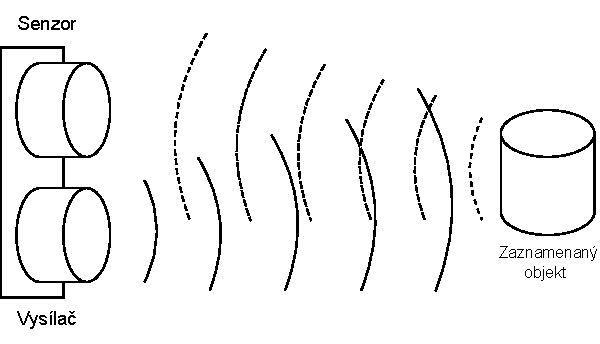
\includegraphics[scale=0.75]{obrazky-figures/ultrasonic.pdf}
	\caption{Ultrazvukový senzor}
	\label{}
\end{figure}

\subsection*{Třícestný senzor pro sledování čáry}
Modul využívá fakt, zě intenzita světla odraženého od povrchu je závislá na barvě dané plochy. Například černá barva pohltí téměř veškeré světlo, naopak bílá téměř vše odrazí. Používáno je infračervené záření, protože není ovlivněno okolními zdroji světla, odráží se od velkého množství materiálů a je přesné. Jedná se o třícestný modul a skládá se tedy ze setu tří vysílačů a senzorů. Pokud vysílač svítí a senzor nezaznamenává dostatečnou intenzitu odraženého světla, znamená to, že byla nalezena černá čára. \cite{embeded_robotics}
Komunikace s mikrokontrolerem je realizována pomocí GPIO vstupů, na které jsou připojeny tři vývody z modulu. Každý z nich reprezentuje jeden set vysílače a senzoru. Jednička na výstupu indikuje, že čára byla detekována.

\subsection*{WS2812 RGB LED}
WS2812 je druh adresovatelných LED diod. Pojmem adresovatelných je myšleno, že není každá dioda připojena k mikrokontroleru zvláště, ale sdílejí jeden datový vodič pro nastavování barev. Prakticky to znamená, že pásek, který může obsahovat i stovky diod je připojený jen pomocí tří vodičů. Těmito vodiči jsou napájení, země a vstupní data. \cite{ws2812}

\begin{figure}[h!]
	\centering
	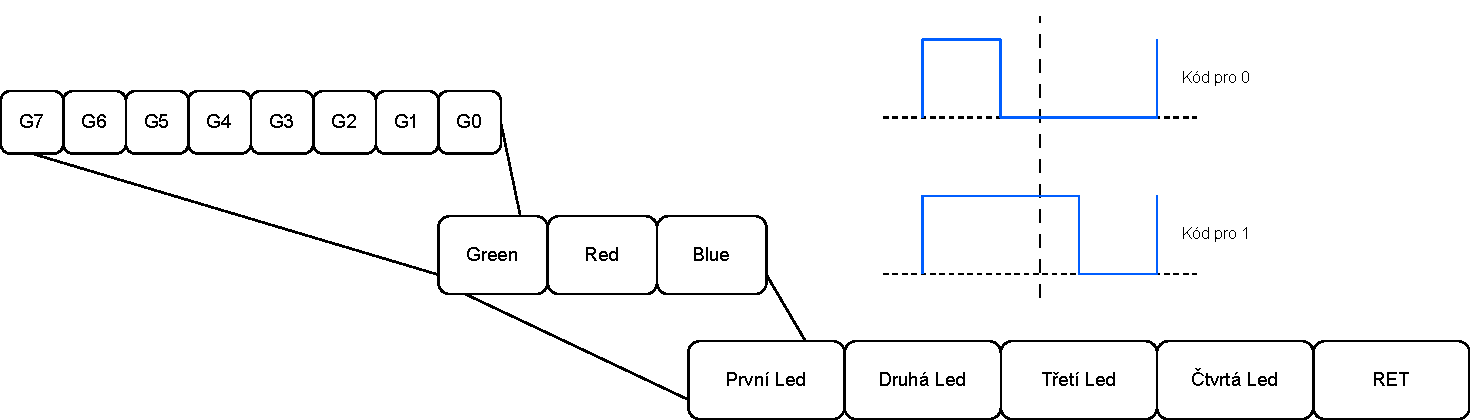
\includegraphics[scale=0.55]{obrazky-figures/ws2812_led.pdf}
	\caption{Komunikační protokol pro WS2812 led}
	\label{}
\end{figure}

Diody jsou na pásku zapojeny sériově. Každá dioda má DIN a DO port. Pokud dioda přijme data, která jí nejsou určená, přeposílá je dále. Komunikace vždy začíná klidovým stavem, datový vodič je v nule. Datové slovo se skládá z 24 bitových bloků pro každou diodu. Blok obsahuje tři osmi bitové hodnoty, jednu pro každou barevnou složku (MSB je posíláno první). Diody pak fungují tak, že přijmou prvních 24 bitů, podle kterých nastaví svou barvu. Tuto část odeberou z datového slova a zbytek přeposílají na výstup. \cite{ws2812}

\section{Raspberry Pi 4b}
Jako mozek celého systému je použit mikropočítač Raspberry Pi. V porovnání s běžně používanými mikrokontroléry, sloužícími pro řízení vestavěných systémů, se jedná o výkonnější hardware, který zvládá i komplexnější operace, jako běh plnohodnotného operačního systému a zpracování obrazu. Konkrétně se jedná o verzi 4 model B s operační pamětí o velikosti čtyř gigabajtů. Tato verze obsahuje 64bitový procesor, ten je potřeba pro spuštění 64 bitového Ubuntu serveru, který je doporučeným operačním systémem pro požití ROS2 na Raspberry Pi.
Komunikace s většinou použitých periferií je uskutečněna pomocí General Purpuse Input Output(GPIO) pinů. Jedná se o číslicové vývody, které podle potřeby můžou fungovat jako vstup i výstup ze zařízení. Některé z nich pak mají ještě speciální funkce, například GPIO 2 a 3 můžou pracovat jako SDA a SCL připojení pro I2C komunikaci.

\begin{figure}[h!]
	\centering
	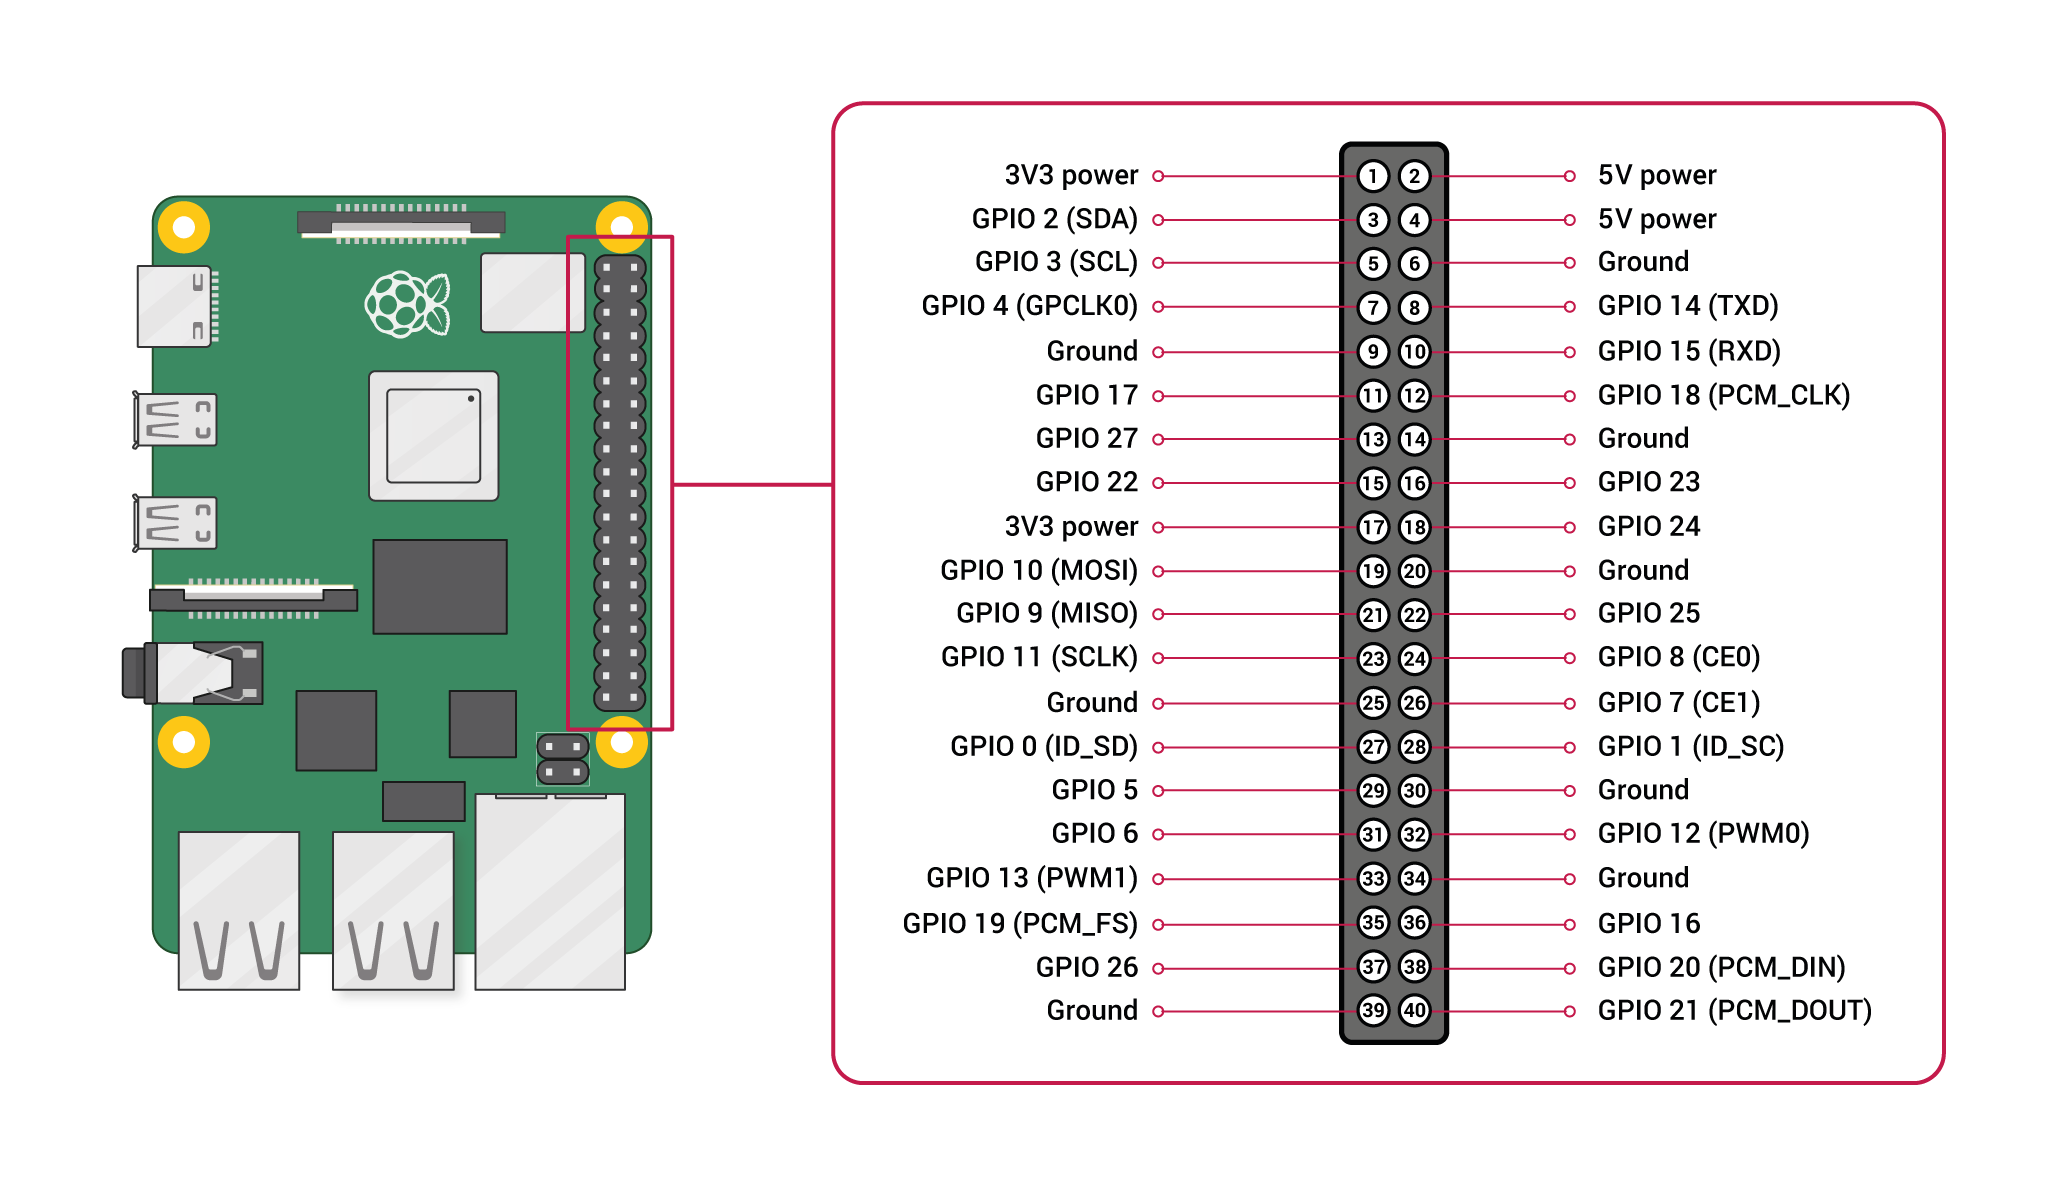
\includegraphics[scale=0.15]{obrazky-figures/gpio_pinout.png}
	\caption{GPIO pinout pro Raspberry Pi}
	\label{}
\end{figure}

\subsection*{Camera}
Přímo k rapsberry pi je připojena oficiální rpi camera v3. Tento modul dokáže nahrávat video až v rozlišení 2304 × 1296 pixelů a 56 snímcích za vteřinu. Avšak pro zpracování, případně analýzu obsahu videa v reálném čase s těmito specifikacemi nemá Raspberry Pi dostatečný výkon. Prakticky budou využity nižší rozlišení a snímkovací frekvence. \cite{rpi_camera}
%opencv

\chapter{Software pro řízení robota}
Jak už bylo řečeno, software poběží na Raspberry Pi. Jako primární programovací jazyk byl zvolen python, protože je jedním z oficiálních jazyků podporovaných ROS2 a také jsou v něm implementovány potřebné knihovny pro ovládání periferií.

\section{Aktuální software}
Robot Adeept AWR 4WD je dodáván s ukázkovým softwarem. Ten je implementován v jazyce Python a využívá knihovny třetích stran sloužící k nízkoúrovňovému ovládání hardwarových komponent. Aby byl robot responzivní je celá implementace řešena s použitím python modulů pro realizaci multithreadingu.

\section{Seznámení s ROS2}
ROS2 je middleware sloužící k vývoji a řízení robotů. Middleware je softwarová vrstva běžící nad operačním systémem. Jejím úkolem je rozšíření operačního systému o další funkcionalitu. Typickou součástí middlewaru bývají knihovny, ovladače, vývojové a monitorovací nástroje. Může také specifikovat doporučené metodologie pro vývoj. ROS2 je již druhá verze tohoto softwaru, která rozšiřuje a opravuje neduhy první verze. Původní ROS1 je považován za de-facto standart pro vývoj robotických aplikací.
Tato práce využívá ROS2 distribuci jménem iron. Distribuce v ROS2 lze popsat jako set operačního systému, knihoven a dalších aplikací, které jsou otestovány a je zaručeno, že jsou navzájem kompatibilní. Velkou výhodou ROS je fakt, že se jedná o open source projekt. Díky tomu kolem něj vznikla velká komunita vývojářů, ale i firem a dalších institucí, které tvoří mnoho souvisejícího obsahu. Existuje tedy velké množství knihoven, dokumentací a návodů které usnadňují vývojářům práci. \cite{ros2_introduction}

\subsection*{Vrstvy ROS2}
Na nejvyšší úrovni, se nachází programátor, který interaguje s klientskými knihovnami pro vývoj ROS2 aplikací. Tyto knihovny jsou oficiálně dvě a to rclpy pro python a rclcpp pro C++. Existují také implementace pro další programovací jazyky (rclc, java, C\#), které jsou však udržovány komunitně. Všechny klientské knihovny pak využívají RCL. To je jádrem celého ROS a obsahuje implementaci všech ros2 funkcionalit. Je napsáno v jazyce C a jeho součástí je rozhraní, pomocí kterého poskytuje svou funkcionalitu ostatním klientským knihovnám. Díky tomuto přístupu se uzly implementované v pythonu budou chovat stejně jako ty implementované v c++. Z toho pak také vyplývá, že uzly implementované na různých klientských knihovnách spolu mohou bez problémů komunikovat.
Poslední vrstvou je data distribution service. DDS je komunikační vrstva implementována na UDP protokolu sloužící k předávání informací mezi procesy. Má charakteristiky systémů reálného času, zajišťuje kvalitu a zabezpečení komunikace. Také umožňuje vyhledávání uzlů bez potřeby centralizovaného serveru (vyhledávání je realizováno s využitím multicastové komunikace, zprávy zasílané mezi jednotlivými uzly pak využívají klasický unicast). \cite{ros2_introduction}

\begin{figure}[h!]
	\centering
	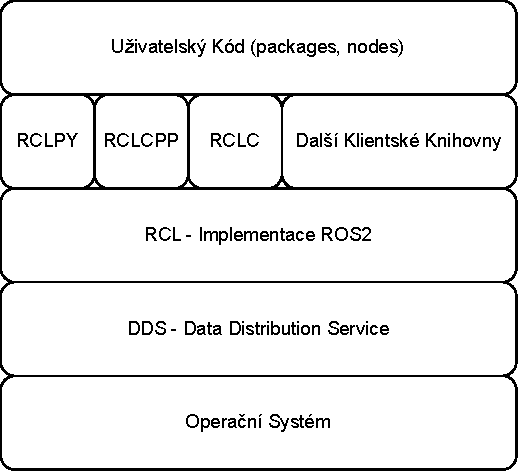
\includegraphics[scale=0.75]{obrazky-figures/ros_layers.pdf}
	\caption{Vrstvy ROS2 systému}
	\label{}
\end{figure}

\subsection*{Vývoj v ROS2}
Nejvyšší organizační jednotkou v ROS2 je workspace. Jedná se o složku, která slouží k organizaci zdrojových souborů, jejich instalaci a následné spouštění. ROS2 se také kvalifikuje jako workspace a před použitím musí být nejprve aktivován. K tomu v linuxu slouží příkaz \verb|source|. Aktivace workspace je akumulativní, to znamená, že v jeden moment může být aktivních několik workspace najednou. Typicky se první aktivuje základní ros2 instalace, která tvoří takzvanou underlay vrstvu. Vývojový workspace aktivovaný jako druhý, se pak nazývá overlay. Pokud má overlay nějaké závislosti, měly by být uspokojeny v underlay.
Zdrojové soubory v rámci workspace jsou pak organizovány do packages. Package může obsahovat zdrojové soubory, knihovny a definice zpráv. Packages na sobě můžou navzájem záviset (např: package která využívá interface závisí na jiné která tento interface definuje). \cite{ros2_introduction}

\begin{figure}[h]
	\begin{forest}
		for tree={
			font=\ttfamily,
			grow'=0,
			child anchor=west,
			parent anchor=south,
			anchor=west,
			calign=first,
			inner xsep=7pt,
			edge path={
				\noexpand\path [draw, \forestoption{edge}] (!u.south west) +(7.5pt,0) |- (.child anchor) \forestoption{edge label};
			},
			before typesetting nodes={
				if n=1
				{insert before={[,phantom]}}
				{}
			},
			fit=band,
			before computing xy={l=15pt},
		}
		[Workspace
			[build {\hspace{3em}\#soubory používané při kompilaci}
			]
			[install {\hspace{2em}\#výsledky kompilace a další soubory potřebné ke spuštění}
			]
			[log {\hspace{4em}\#logy z kompilace}
			]
			[launch {\hspace{2.5em}\#launch soubory}
			]
			[src {\hspace{4em}\#packages}
				[package\_name {\hspace{2em}\#příklad jak vypadá python package}
					[package\_name {\hspace{2em}\#zdrojové python soubory}
					]
					[resource
					]
					[test
					]
					[package.xml {\hspace{1em}\#metadata infromace o package}]
					[setup.cfg {\hspace{2em}\#konfigurace pro manuální spouštění uzlu}]
					[setup.py {\hspace{2.5em}\#instrukce pro kompilátor jak nainstalovat package}]
				]
			]
		]
	\end{forest}
  	\caption{Struktura ROS2 Workspace}
	\label{}
\end{figure}

\subsubsection*{Node}
Celý ROS2 systém je složený z uzlů (node), které mezi sebou navzájem komunikují. Každý uzel je vlastní výpočetní jednotka, která by měla plnit jeden specifický úkol. Tento přístup je podobný objektově orientovanému návrhu a ROS2 jej také využívá. Implementačně je uzel objekt, který dědí ze třídy \verb|Node|.
Uzly v ROS2 většinou nepotřebují běžet permanentně, ale pouze v monentě, kdy nastane nějaká událost, kterou je potřeba obsloužit. Z toho důvodu existuje v ROS2 metoda \verb|spin()|, která uspí vykonávání uzlu, dokud jej není potřeba opět využít. Aby ROS2 šetřil výpočetní prostředky, využívá dva přístupy k určení, kdy bude potřeba uzel vzbudit. Prvním je iterative execution, ten se používá u uzlů, které vykonávájí svou činnost pravidelně na nějaké předem dané frekvenci. Například se může jednat o výpočetní uzel, který pravidelně každých x mikrosekund provede výpočet podle hodnot senzorů a odešle výsledek.
Druhý je event oriented execution. Zde dochází k vyvolání řídícího cyklu jako důsledek nějaké události, typicky se jedná od příchozí zprávu z subscription, service nebo action. Frekvenci spouštění těchto uzlů pak lze odvodit od frekvence příchozích zpráv. Typicky se může jednat o uzel přijímající snímky z kamery na kterých provede výpočet a vrátí odpověď. Frekvence výpočtu je dána příchozími snímky, pokud snímky přestanou přicházet, uzel se nebude spouštět. \cite{ros2_introduction} \cite{ros2_documentation}

\begin{algorithm}[h!]
	\label{}
	\caption{\textsc{Definice a použití Node objektu}}
	
	\DontPrintSemicolon
	\SetAlgoNoLine
	\SetAlgoNlRelativeSize{-1}
	\SetNlSty{}{}{:}
	\SetNlSkip{-1.1em}
	
	\BlankLine \Indp\Indpp
	
	\texttt{class CustomNode(Node):}\;
	\Indp\Indp
	\texttt{def \_\_init\_\_(self):}\;
	\Indp\Indp
	\texttt{super().\_\_init\_\_('node\_name')}\;
	\Indm\Indm\Indm\Indm
	
	\BlankLine
	
	\texttt{def main(args):}\;
	\Indp\Indp
	\texttt{rclpy.init(args=args)}\;
	\texttt{node = CustomNode()}\;
	\texttt{rclpy.spin(node)}\;
	\texttt{node.destroy\_node()}\;
	\texttt{rclpy.shutdown()}\;
\end{algorithm}

\subsubsection*{Topic}
Je základním a také nejčastěji používaným způsobem pomocí kterého spolu ROS2 uzly komunikují. Topic si lze představit jako analogii hardwarové sběrnice. Prakticky se jedná o přesně pojmenované místo, do kterého může n uzlů posílat data (Publish) a m poslouchat co bylo posláno (Subscribe). Zprávy posílané do topicu mají přesný formát a jsou posílány asynchronně. Příkladem použití může být topic, do nějž posílá data uzel ovládající kameru a několik dalších uzlů které tyto data potřebují jej mohou číst. \cite{ros2_introduction}

\begin{algorithm}[h!]
	\label{}
	\caption{\textsc{Subsrciber Node}}
	
	\DontPrintSemicolon
	\SetAlgoNoLine
	\SetAlgoNlRelativeSize{-1}
	\SetNlSty{}{}{:}
	\SetNlSkip{-1.1em}
	
	\BlankLine \Indp\Indpp
	\texttt{self.create\_subscription(Interface, "topic\_name", self.callback\_function, queue\_size)}\;
	
	\BlankLine
	\texttt{def callback\_function(self, msg):}\;
	\Indp\Indp
	\texttt{value = msg.item}\;
\end{algorithm}
Tento kód ukazuje, jak se může uzel přihlásit v odebírání zpráv z topicku. Nejprve je potřeba (typicky v konstruktoru třídy) zavolat zděděnou metodu sloužící k inicializaci nějaké ROS2 funkcionality. V tomto případě se jedná o \verb|create_subscription|. Jako parametry potřebuje jméno, interface, callback funkci a délku fronty. Inteface definuje formát zpráv a délka fronty je použita v případě, že uzel nezvládá přijímat zprávy dostatečně rychle. Callback funkce je pak zavolána pokaždé když do topicku přijde nová zpráva. Druhým parametrem callback funkce je předán objekt, který ve svých atributech obsahuje hodnoty dané zprávy. \cite{ros2_documentation}

\begin{algorithm}[h!]
	\label{}
	\caption{\textsc{Publisher Node}}
	
	\DontPrintSemicolon
	\SetAlgoNoLine
	\SetAlgoNlRelativeSize{-1}
	\SetNlSty{}{}{:}
	\SetNlSkip{-1.1em}
	
	\BlankLine \Indp\Indpp
	\texttt{self.publisher = self.create\_publisher(Interface, "topic\_name", queue\_size)}\;
	
	\BlankLine
	\texttt{output = Interface()}\;
	\texttt{output.item = some\_value}\;
	\texttt{self.publisher.publish(output)}\;
\end{algorithm}
Odesílání zpráv do topicu demonstruje tento kód. Jeho struktura je podobná předchozímu příkladu. Odeslání zprávy demonstrují řádky 2--4. Nejprve dojde k inicializaci objektu interface, stejného datového typu jako ten, který používá topic. Tento objekt je následně naplněn daty a pomocí metody \verb|publish()| předem vytvořeného publisheru odeslán. \cite{ros2_documentation}

\subsubsection*{Service}
Sevice funguje na stejném principu jako klient--server komunikace známá z počítačových sítí. Jedná se tedy o synchronní komunikaci, kde jeden uzel poskytuje nějakou službu a ostatní si na ni mohou poslat požadavek. Od service uzlu se typicky předpokládá okamžitá odpověď, aby nedošlo k narušení řídícího cyklu volajícího uzlu. \cite{ros2_introduction}
\newpage

\begin{algorithm}[h!]
	\label{}
	\caption{\textsc{Service server}}
	
	\DontPrintSemicolon
	\SetAlgoNoLine
	\SetAlgoNlRelativeSize{-1}
	\SetNlSty{}{}{:}
	\SetNlSkip{-1.1em}
	
	\BlankLine \Indp\Indpp
	
	\texttt{self.srv = self.create\_service(Interface, "service\_name", self.callback\_function)}\;
	\BlankLine
	\texttt{def callback\_function(self, request, response):}\;
	\Indp\Indp
	\texttt{value = request.item}\;
	\texttt{response.item = some\_value}\;
	\texttt{return response}\;
	
\end{algorithm}
Změnou oproti předchozím příkladům je přidání nového parametru do callback funkce. Tato funkce má nyní dva důležité parametry, request a response. Request obsahuje konkrétní hodnoty požadavku na server a response je potřeba naplnit výsledky a vrátit z funkce. \cite{ros2_documentation}

\begin{algorithm}[h!]
	\label{}
	\caption{\textsc{Service client}}
	
	\DontPrintSemicolon
	\SetAlgoNoLine
	\SetAlgoNlRelativeSize{-1}
	\SetNlSty{}{}{:}
	\SetNlSkip{-1.1em}
	
	\BlankLine \Indp\Indpp
	
	\texttt{self.cli = self.create\_client(Interface, "service\_name")}\;
	\texttt{while not self.cli.wait\_for\_service(timeout\_sec=1.0):}\;
	\Indp\Indp
	\texttt{pass}\;
	\Indm\Indm

	\BlankLine
	\texttt{def send\_request(self):}\;
	\Indp\Indp
	\texttt{self.req = Interface.Request()}\;
	\texttt{self.req.item = some\_value}\;
	\texttt{self.future = self.cli.call\_async(self.req)}\;
	\texttt{rclpy.spin\_until\_future\_complete(self, self.future)}\;
	
	\BlankLine
	\texttt{response = self.future.result()}\;
	\texttt{value = response.item}\;
\end{algorithm}
Service client narozdíl od topic subscriberu závisí na tom, aby existoval server, který je schopný odpovídat na jeho požadavky. Tato podmínka vyplývá z faktu, že service server by měl odpovídat na dotazy téměř okamžitě a service klient tedy předpokládá, že vždy dostane odpověď. Pokud by neexistoval server, klient by při požadavku skončil v nekonečném čekání. Proto je hned v konstruktoru implementována kontrola, které nedovolí vytvoření uzlu dokud není přítomen server. Čekání na odpověď od serveru, je pak implementována pomocí funkce \verb|spin_until_future_complete()| \cite{ros2_documentation}

\subsubsection*{Action} %cite web documentation
Jedná se o rozšířenou verzi service. Akce z pravidla vykonává déle trvající požadavek. Například provedení řídícího manévru robota, který je prováděn v reálném světě a z pohledu uzlu se nejedná o krátkodobou záležitost. Akce, na rozdíl od service, dokáže v průběhu vykonávání své činnosti odesílat průběžné aktualizace o aktuálním stavu zpět volajícímu uzlu. Implementačně akce funguje jako dva service a jeden topic. Cílový (goal) service slouží k zaslání požadavku na server a jeho potvrzení. Výsledkový (result) pak vrací výsledek operace. V průběhu akce pak server posílá aktualizace do topicu. \cite{ros2_introduction}
\newpage

\begin{algorithm}[h!]
	\label{}
	\caption{\textsc{Action server}}
	
	\DontPrintSemicolon
	\SetAlgoNoLine
	\SetAlgoNlRelativeSize{-1}
	\SetNlSty{}{}{:}
	\SetNlSkip{-1.1em}
	
	\BlankLine \Indp\Indpp
	
	\texttt{self.action\_server = ActionServer(self, Interface, "action\_name", self.callback\_function)}\;
	
	\BlankLine
	\texttt{def callback\_function(self, goal\_handle):}\;
	\Indp\Indp
	\texttt{goal\_handle.request.item}\;
	
	\BlankLine
	\tcp{odeslání zpětné vazby volajícímu}
	\texttt{feedback = Interface.Feedback()}\;
	\texttt{feedback.item = some\_value}\;
	\texttt{goal\_handle.publish\_feedback(feedback)}\;
	
	\BlankLine
	\tcp{úspěšné ukončení požadavku}
	\texttt{goal\_handle.succeed()}\;
	\texttt{result = Interface.Result()}\;
	\texttt{result.item = some\_value}\;
	\texttt{return result}\;
\end{algorithm}
Action server využívá stejné postupy jako předchozí ukázky, pouze jich kombinuje více dohromady. V rámci callback funkce může odesílat průběžně zpětnou vazbu a nakonec jako návrat z funkce předá výsledek. \cite{ros2_documentation}

\begin{algorithm}[h!]
	\label{}
	\caption{\textsc{Action client - zaslání požadavku}}
	
	\DontPrintSemicolon
	\SetAlgoNoLine
	\SetAlgoNlRelativeSize{-1}
	\SetNlSty{}{}{:}
	\SetNlSkip{-1.1em}
	
	\BlankLine \Indp\Indpp
	
 	\texttt{self.action\_client = ActionClient(self, Interface, "action\_name")}\;
 	
 	\BlankLine
 	\texttt{def send\_goal(self):}\;
 	\Indp\Indp
 	\texttt{goal\_msg = Servo.Goal()}\;
 	\texttt{goal\_msg.item = some\_value}\;
 	\texttt{self.action\_client.wait\_for\_server()}\;
 	\texttt{self.goal\_future = self.action\_client.send\_goal\_async(goal\_msg, self.feedback\_callback\_function)}\;
 	\texttt{self.goal\_future.add\_done\_callback(self.response\_callback\_function)}\;
	\Indm\Indm
    
\end{algorithm}
Při pohledu na implementaci action klienta lze dobře vidět vnitřní implementace akcí. První funkce \verb|send_goal()| vypadá podobně jako service client. Dojde zde k zaslání požadavku na server a následné čekání na odpověď. Čekání tentokrát není aktivní, aby nedošlo k uváznutí, ale je realizováno pomocí callback funkce. Součástí dotazu je také topic pro zasílání aktualizací. \cite{ros2_documentation}
\newpage

\begin{algorithm}[h!]
	\label{}
	\caption{\textsc{Action client - reakce na přijmutí nebo zamítnutí požadavku}}
	
	\DontPrintSemicolon
	\SetAlgoNoLine
	\SetAlgoNlRelativeSize{-1}
	\SetNlSty{}{}{:}
	\SetNlSkip{-1.1em}
	
	\BlankLine \Indp\Indpp
	
	\texttt{def response\_callback\_function(self, future):}\;
	\Indp\Indp
	\texttt{goal\_handle = future.result()}\;
	\texttt{if not goal\_handle.accepted:}\;
	\Indp\Indp
	\texttt{return}\;
	\Indm\Indm
	
	\BlankLine
	\texttt{self.result\_future = goal\_handle.get\_result\_async()}\;
	\texttt{self.result\_future.add\_done\_callback(self.result\_callback\_function)}\;
	\Indm\Indm
	
\end{algorithm}
Druhá \verb|response_callback_function| pak zpracuje výsledek požadavku (přijmutí nebo zamítnutí) a pošle požadavek na result service, který nakonec vrátí výsledek. \cite{ros2_documentation}

\begin{algorithm}[h!]
	\label{}
	\caption{\textsc{Action client - callback funkce}}
	
	\DontPrintSemicolon
	\SetAlgoNoLine
	\SetAlgoNlRelativeSize{-1}
	\SetNlSty{}{}{:}
	\SetNlSkip{-1.1em}
	
	\BlankLine \Indp\Indpp
	
	\BlankLine
	\texttt{def feedback\_callback\_function(self, msg):}\;
	\Indp\Indp
	\texttt{feedback = msg.feedback}\;
	\texttt{value = feedback.item}\;
	\Indm\Indm
	
	\BlankLine
	\texttt{def result\_callback\_function(self, future):}\;
	\Indp\Indp
	\texttt{result = future.result().result}\;
	\texttt{value = result.item}\;
	
\end{algorithm}

\subsubsection*{Interface}
Interface slouží k určení přesného formátu jednotlivých zpráv, které jsou posílány mezi uzly. ROS2 obsahuje mnoho již vytvořených a vývojáři po celém světě používaných formátů. Tento přístup podporuje znovupoužitelnost vytvořeného kódu a šetří práci. Díky tomu může být software pro ovládání konkrétního kusu hardware naimplementován pouze jednou s využitím standartního rozhraní a všichni ostatní jej pak mohou využít ve svých systémech.
Pokud však standartní interface nevyhovuje potřebám, lze si naimplementovat vlastní. K definici konkrétního formátu slouži tři druhy souborů. \cite{ros2_introduction}

Prvním jsou \verb|.msg| zprávy. Tento formát je využívám topicy. Jedná se o seznam, kde je každá položka definována jako dvojice datový typ a název (případně komentář).
\begin{verbatim}
	int32 angle #comment
	string direction
\end{verbatim}

Druhým je \verb|.srv|. Slouží pro definici request/response zpráv pro komunikaci se servicem. Tento soubor obsahuje dvě části, požadavek a odpověď, každá je tvořena seznamem položek a jsou odděleny řádkem \verb|---|. 
\begin{verbatim}
	int32 a
	int32 b
	---
	int64 sum
\end{verbatim}

Poslední je \verb|.action| soubor. Slouží pro komunikaci s action serverem. Definice se skládá ze tří seznamů, jeden pro požadavek, druhý pro odpověď a poslední pro stavové aktualizace.
\begin{verbatim}
	float32 goal_angle
	---
	bool response
	---
	float32 current_angle
\end{verbatim}

\subsubsection*{Parametry}
ROS2 uzly lze spouštět s parametry. Typicky slouží k nastavení hodnot (předání konfiguračního souboru) za běhu programu bez potřeby zásahu do zdrojových kódů. Příkladem může uzel, sloužící k obsluze periferního zařízení a parametrem jsou mu předány čísla GPIO pinů na které je dané zařízení připojeno. \cite{ros2_introduction}

\begin{algorithm}[h!]
	\label{}
	\caption{\textsc{Parameters}}
	
	\DontPrintSemicolon
	\SetAlgoNoLine
	\SetAlgoNlRelativeSize{-1}
	\SetNlSty{}{}{:}
	\SetNlSkip{-1.1em}
	
	\BlankLine \Indp\Indpp
	
	\tcp{deklarace parametru, typicky v konstruktoru}
    \texttt{self.declare\_parameter('parameter\_name', 'default\_parameter\_value')}\;
	
	\BlankLine
	\tcp{získání hodnoty parametru}
	\texttt{param = self.get\_parameter('parameter\_name').get\_parameter\_value().string\_value}\;
	
	\BlankLine
	\tcp{nastavení hodnoty parametru}
	\texttt{new\_param = rclpy.parameter.Parameter(}\;
	\Indp\Indp
	\texttt{'parameter\_name',}\;
	\texttt{rclpy.Parameter.Type.STRING,}\;
	\texttt{'default\_parameter\_value'}\;
	\Indm\Indm
	\texttt{)}\;
	\texttt{new\_param\_list = [new\_param]}\;
	\texttt{self.set\_parameters(new\_param\_list)}\;

\end{algorithm}

\subsubsection*{Launch File}
ROS2 systém se skládá z velkého množství navzájem komunikujících uzlů, a protože spouštění každého uzlu zvlášť by bylo pracné a zdlouhavé, existují launch soubory, které tuto práci usnadňují. Tyto soubory můžou být napsány v pythonu, yaml nebo xml. Čtyři hlavní úkoly, které launch soubory plní, jsou spouštění uzlu, volání dalšího launch souboru, nastavení parametrů a proměnných prostředí. Prakticky se launch soubory píší minimálně na dvou úrovních. Na nižší úrovni se využívají jako součást package, kde slouží k spouštění jednotlivých uzlů. Jejich úkolem je nastavit uzel tak, aby nebylo potřeba modifikovat zdrojový kód. Typicky tak nastavuje správný namespace, předávají parametry, konfigurační soubory a případně dochází k přemapování jména topicu. Launch soubory vyšších úrovní pak slouží ke spuštění několika uzlů zároveň a využívají k tomu launch soubory nacházející se v packages. \cite{ros2_introduction}

\begin{algorithm}[h!]
	\label{}
	\caption{\textsc{Launch file}}
	
	\DontPrintSemicolon
	\SetAlgoNoLine
	\SetAlgoNlRelativeSize{-1}
	\SetNlSty{}{}{:}
	\SetNlSkip{-1.1em}
	
	\BlankLine \Indp\Indpp
	
	\texttt{def generate\_launch\_description():}\;
	\Indp\Indp
	\texttt{return LaunchDescription([}\;
	\Indp\Indp
	\tcp{spuštění konkrétního uzlu}
	\texttt{Node(}\;
	\Indp\Indp
	\texttt{package='package\_name',}\;
	\texttt{executable='node\_name',}\;
	\texttt{namespace='namespace\_name',}\;
	\texttt{parameters=[\{}\;
	\Indp\Indp
	\texttt{'param\_name' : param\_value,}\;
	\Indm\Indm
	\texttt{\}]}\;
	\Indm\Indm
	\texttt{),}\;
	\texttt{Node(}\;
	\Indp\Indp
	\texttt{package='package\_name',}\;
	\texttt{executable='node\_name',}\;
	\texttt{remappings=[}\;
	\Indp\Indp
	\texttt{('topic\_name', 'different\_topic\_name'),}\;
	\Indm\Indm		
	\texttt{]}\;
	\Indm\Indm	
	\texttt{),}\;
	\tcp{zavolání dalšího launch souboru}
	\texttt{IncludeLaunchDescription(}\;
	\Indp\Indp
	\texttt{PythonLaunchDescriptionSource([}\;
	\Indp\Indp
	\texttt{PathJoinSubstitution([}\;
	\texttt{FindPackageShare('package\_name'),}\;
	\Indp\Indp
	\texttt{'launch',}\;
	\texttt{'node\_name.py'}\;
	\Indm\Indm	
	\texttt{])}\;
	\Indm\Indm	
	\texttt{]),}\;
	\Indm\Indm	
	\texttt{)}\;
	\Indm\Indm	
	\texttt{])}\;
		
\end{algorithm}


\subsection*{Formáty pro popis Robotů}
V robotice se často objevuje potřeba definovat strukturu a fyzikální vlastnosti robotů, objektů případně prostředí, ve kterém se nachází. Nejzjevnějším případem jsou simulátory ale existují i jiné použítí kde programy potřebují znát aktuální stav, odometrii robota, a k tomu je nejprve potřeba znát jeho stukturu.

\subsubsection*{Unified Robotics Description Format}


\subsubsection*{XML Macro}
Xacro lze použít na jakékoli XML soubory, ale primárně se používá k generování URDF souborů. Cílem tohoto formátu je zjednodušení URDF souborů, které se při popisu složitějších robotů stávají dlouhé a náchylné na chyby. Xcarco tedy přidává funkce sloužící k eliminaci těchto nedostatků. 
První z nich je možnost definovat konstanty, v urdf se často opakují stejné hodnoty na několika místech, jednoduchým případem může být definice vizuální a kolizní části <link> elementů které bývají často totožné. 
\begin{verbatim}
	<xacro:property name="wheel_radius" value="0.035" />
\end{verbatim}
Na konstanty pak navazuje vkládání matematických výrazů, místo statických hodnot.
\begin{verbatim}
	<cylinder radius="${wheel_diameter/2}" length="0.1"/>
\end{verbatim}
Hlavní funkcionalitou tohoto formátu jsou však makra. Ty umožňují zaobalit blok kódu a přiřadit mu identifikátor pomocí kterého lze takové makro vkládat na další místa v kódu. 
Makra mohou brát na vstupu také parametry. V těle makra lze pak tyto parametry vkládat a v kombinaci s matematickými výrazy vytvářet komplexní definice.
\begin{verbatim}
	<xacro:macro name="identificator" params="name mass:=default_value">
\end{verbatim}
Posledním rozšířením které xacro oproti urdf prináší je možnost rozdělení definice robota do více souborů.
\begin{verbatim}
	<xacro:include filename="components.xacro"/>
\end{verbatim}

\subsubsection*{Simulation Description Format}

SDF je formát založený na XML. Jak z názvu vyplývá, slouží k popisu robotů, ale také světů ve kterých se budou následně pohybovat. Jedná se o primární formát využívaný Gazebo simulátorem.

\subsubsection*{Rviz2}

\subsection{Simultaneous Localization And Mapping}



\subsection{Navigation 2}

\subsection{Geometric Transformation Subsystem}
Jedná se o subsystém ros2, který realizuje geometrické transformace mezi jednotlivými částmi robota.
Vztah mezi dvěma objekty lze definovat pomocí posunu (translation) a otočení (rotation). Matematicky jsou tyto složky reprezentovány maticemi, které po spojení vytváří výslednou transformační matici. Vzhledem k tomu, že roboti se skládají z velkého množství částí, které jsou na sebe navzájem zavěšeny a zároveň se jejich relativní pozice neustále mění, není vhodné počítat tyto vztahy manuálně a proto existuje TF.

Základním prvkem se kterým TF pracuje je takzvaný frame, neboli rám. Rám reprezentuje nějakou část robota jako senzor, kolo a podobně. Tyto rámy jsou uspořádány do stromové struktury, kde každý uzel má vždy jednoho předka. Kořenem robota je z pravidla \verb|base_link|, který se nachází v jeho středu. Dalším běžným rámem je \verb|odom|. Ten reprezentuje vztah mezi aktuální pozicí robota a počátkem souřadného systému.

Pro předávání dat mezi uzly jsou využívány dva topicy.
\begin{itemize}
	\item {\verb|/tf| - dynamické transformace pro komponenty připojené přes serva, motory}
	\item {\verb|/tf_static| - statické transformace pro komponenty pevně připevněné na jiné části}
\end{itemize} 
ROS2 uzly neinteragují s těmito topicy stejně jako s běžnými topicky ale pomocí speciálních objektů k tomu sloužícím. Pro zasílání nových dat do TF systému slouží \verb|TransformBroadcaster|. Ten se používá vesměs stejně jako klasický publisher.
Pro získání dat z tf systému pak slouží \verb|TransformListener|. Ten neslouží k jednoduchému čtení zpráv posílaných v topicu, ale umožňuje dotazování se tf systému na konkrétní transformace. Dotaz se skládá z specifikování dvou rámců, mezi kterými je transformace hledána. Tyto dva rámce nemusí být v tf stromu přímí potomci. Cesta od jednoho k druhému může vést přes několik uzlů, ale dokud jsou navzájem dosažitelné, tak tf vrátí výslednou transformaci. Druhou částí dotazu je čas, ten je potřebný protože, pokud je cesta mezi rámy delší může se i během několika milisekund výrazně změnit výsledná transformace a použití aktuálního času tak není vhodné. Specifikování času také umožňuje získávat pozice z minulosti. 

\chapter{Implementace}


\section{Uzly pro řízení komponent}

\subsection*{Komponenty součástí adeept kitu}

\subsubsection*{Motory}
Robot disponuje čtyřmi stejnosměrnými motory. Řizení je tedy realizováno differenciálním způsobem. 
V ROS systému je ovládání motoru realizováno uzlem \verb|dc_motor_node|. Tento uzel přímo ovládá GPIO piny, pomocí kterých řídí h-bridge obvod. Co se týče interakce s ros2 systémem, tento uzel poslouchá topic jménem \verb|cmd_vel| command velocity. Jedná se o standartní topic pro posílání příkazu na pohyb robota. Zprávy v tomto topicu jsou typu Twist. Pro robota s differenciálním pohonem je tedy důležitá lineární x složka a angulární z. Pomocí nich lze spočítat výsledná rychlost otáčení pro kola na jedné a druhé straně.

$$\omega_L = \frac{V - \omega * b/2}{r}$$
$$\omega_R = \frac{V + \omega * b/2}{r}$$

\noindent Kde $\omega_L$ a $\omega_R$ jsou výsledné rychlosti motorů v $[rad/s]$. $V$ je zadaná lineární a $\omega$ angulární složka v $[m/s] a [rad/s]$. $b$ je rozpětí mezi koly a $r$ poloměr kola v $[m]$.

%problémy, optimalizace

\subsubsection*{Servo}
Tento robot využívá pouze jedno servo a to na ovládání náklonu kamery. Toto servo je řízeno pomocí pwm signálu který generuje PCA9685. V softwaru je k jeho řízení využita knihovna \verb|Adafruit_PCA9685|. Vzhledem k tomu, že použité servo má větší rozsah pohybu, než kolik je místa pro kameru, zajišťuje uzel kontrolu minimálního a maximálního natočení aby nedošlo k poškození robota. Z pohledu ROS2 systému tento uzel demonstruje jednoduchý action server. Server příjme požadavek, postupně otáčí servo do cílové pozice a průběžně odesílá informaci o aktuálním úhlu serva.

\subsubsection*{Kamera}
Zachytávání snímků kamery je realizováno pomocí knihovny OpenCV. Aby bylo možno dosáhnout relativně krátké odezvy při přehrávání obrazu je použito nižší rozlišení a snímkovací frekvence než to co použitá kamera zvládá. V základním configu je použito rozlišení 960 na 540 pixelů a snímkovací frekvence 20hz.
Pro přenos snímků v ROS2 systému je použita zpráva vestavěného typu \verb|CompressedImage|. Před odesláním jsou ještě data zakódována do jpeg formátu pomocí nástrojů opencv.
Před použitím CompressedImage formátu bylo experimentováno také s \verb|Image|. Tato zpráva obsahuje více rozšiřujících informací o přenášeném obrázku jako jeho rozměry, použité kódování a podobně. Na první pohled se tedy zdá jako vhodnější formát. Protože se však jedná o snímky kamery přenášené mezi dvěma různými zařízeními pomocí wifi připojení přináší tento objemově větší formát příliš velké zpoždění, které překonává použitelné hranice pro streamování. Na počátku vývoje byl použit ještě třetí možný přístup, který však nevyužívá ROS2 funkcionality a proto byl později změněn. Tím je zakódování přenášených snímků do \verb|base64| formátu a následné přenesení jako jednoduchou string zprávu. Tento přístup se ukázal jako zcela funkční a dosahující podobných výsledků ve zpoždění jako má \verb|CompressedImage|.
 
\subsubsection*{Ultrazvukový senzor}
Ovládání ultrazvukového senzoru je relativně jednoduché a je tedy realizováno pomocí práce s GPIO piny. Získání aktuální vzdálenosti se skládá z odeslání pulzu na trig pin. Následně se počká dokud senzor nezačne na echo pin odesílat odpověď. V ten moment se uloží časová značka a počká se dokud se echo pin nevrátí zpět na nízkou hladinu. Pak se uloží druhá značka. Interval mezi těmito dvěma momenty lze následně přepočítat na vzdálenost.

Do ROS2 systému tento uzel odesílá kromě pravidelného updatu aktuální vzdálenosti také dvě další informace. Tou první je jednoduché varování o detekci překážky nacházející se přímo před robotem. Druhá zpráva pak doplňuje tu první v ohledu detekování překážek které můžou stále vést ke kolizi ale senzor je již nedetekuje. 

\begin{figure}[h!]
	\centering
	\begin{minipage}[c]{0.5\textwidth}
		\centering
		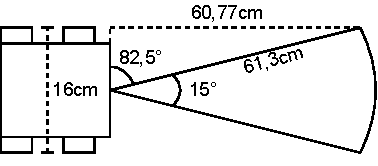
\includegraphics[scale=1.0]{obrazky-figures/ultrasonic_blind_spot.pdf}
	\end{minipage}%
	\begin{minipage}[c]{0.5\textwidth}
			$$\cos(82.5^\circ) = \frac{8\text{cm}}{\text{prepona}} \Rightarrow 61.3\text{cm}$$
			$$\sin(82.5^\circ) = \frac{\text{protilehla}}{61.3\text{cm}} \Rightarrow 60.77\text{cm}$$
	\end{minipage}
	\caption{}
	\label{}
\end{figure}

V tomto případě se jedná o překážky které zmizí ze skeneru ve vzdálenosti menší než 61cm ale ještě nejsou detekovány klasickým způsobem, který informuje o překážkách ve vzdálenosti menší než např: 20cm. Druhá zpráva tedy informuje o tom, že nějaká překážka zmizela ze radaru v této potenciálně nebezpečné vzdálenosti.

%čtení, detekce překážek

\subsubsection*{Sledování čáry}
%not much to say

\subsection*{Rozšíření}
\subsubsection*{Nabíjení}
V originální konfiguraci je napájení realizováno pomocí dvou sériově zapojených 18650 baterií. V tomto zapojení baterie poskytují napájení až 8V a 4A. Součástí adeept kitu jsou kolébky na baterie, které je přímo připojí k zátěži. Nabíjení baterií je tedy realizováno externě. Protože je tento přístup nepohodlný, prvním rozšířením robota je přidání bms a nabíjecí desky. 
Nejrozšířenějším způsobem nabíjení 18650 baterií je deska s čipem TP4056. Tyto desky jsou hojně dostupné, v různých konfiguracích s různými vstupy napájení a ochranami. Problémem je, že tyto desky jsou vhodné pro nabíjení jedné 18650 baterie. Potenciálně lze použít více desek na nabíjení baterií v paralelním zapojení. Ale pro sériově zapojené baterie jsou tyto desky nevhodné.
Lepší přístup je tedy přes využití Battery Management System. Jedná se o desku zajištující ochranu baterií a obsahuje také bod pro připojení mezibodu mezi bateriemi aby mohla správně balancovat nabíjení jednotlivých baterií. V kombinaci s touto deskou se dále využije samotná nabíjecí deska, ta musí dodávat dvojnásobné napětí protože seriové zapojení napětí sčítá.

\begin{figure}[h!]
	\centering
	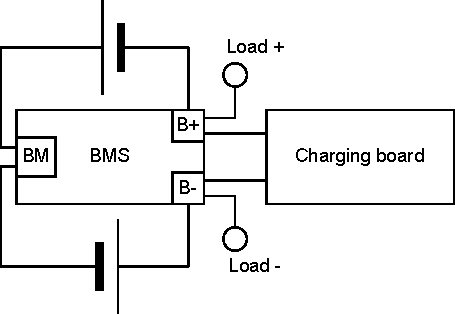
\includegraphics[scale=0.75]{obrazky-figures/battery_circuite.pdf}
	\caption{Zapojení BMS a nabíjecí desky}
	\label{}
\end{figure}

\subsubsection*{Inertial Mesurement Unit - IMU}
Druhým rozšířením oproti originální stavebnici je přidání IMU senzoru. Konkrétně se jedná o model MPU5060. Ten disponuje tří osým akcelerometrem a gyroskopem. Ve výsledném systému pracují s daty z imu dva uzly. Tím prvním je klasický uzel na jeho ovládání, ten využívá knihovnu třetí strany \verb|mpu-5060 dopln|. Nejprve je potřeba vyčistit data. Přímo v hardwaru je implementována dolní propusť, která se nastavuje zápisem do registru \verb|register|. Softwarově lze získaná data zprůměrovat mezi více vzorky a taky je každé čtení upraveno o kalibrační offset, protože senzor i ve statické pozici čte malé hodnoty. Výsledná data pak uzel odesílá kromě klasického Twist topicu také jako odometrii do tf systému.

Druhým uzlem využívajícím tyto data je \verb|motor controller|. Tento uzel zajišťuje přesné ovládání robota. Konkrétně využívá data z gyroskopu aby zajistil otočení robota o konkrétní úhel.

\subsubsection*{Light Detection And Ranging - Lidar}
Posledním a zároveň nejzajímavějším rozšířením je lidar senzor. Jedná se o senzor ze skupiny senzorů pro určování vzdálenosti. Konkrétním použitým modelem je \verb|dopln|. Jendá se o 360 stupnový senzor. Je tedy skvělý pro mapování prostoru, v němž se robot nachází a případně také navigaci.

\section{Řízení robota na vyšší úrovni}
Kromě manuálního ovládání robota 

\subsection{Pomocný uzel pro přesné otáčení robota}
Vzhledem k tomu že použité motory nejsou opatřeny enkodéry, je, bez využití dalších senzorů, jakékoli otáčení velice nepřesné. Motorům lze samozřejmě zadat konkrétní rychlost na určitý časový interval a dostat se tak na přibližně správnou orientaci. Ale opravdu se jedná jen o přibližný úhel z důvodů externích vlivů a nepřesností. Například setrvačnost hraje velkou roli při otáčení o úhly menší než 90° nebo při vyšším využití prostředků mikrokontroleru můžou být reakce na příkazy zpožděné.
Proto byl vytvořen tento uzel, který využívá gyroskopická data z imu senzoru, aby zajistil, že se robot  může v případě potřeby otáčet o přesně dané úhly. V ROS2 systému se jedná o action server. Přijímá požadavky a následně zasílá příkazy na \verb|cmd\_vel| topic. Podle hodnot získaných z imu pak postupně snižuje rychlost otáčení v závislosti na vzdálenosti od cílového úhlu. Z pohledu demonstrace ROS2 funkcionality tento uzel využívá pokročilejší funkce action serveru mezi které patří možnost předat action serveru vlastní callback funkce pro určité události. Ve většině případů se využívá pouze execute callback ve kterém by měla proběhnout většina funkcionality daného action serveru. Tento konkrétní uzel však potřebuje pro své správné fungování data z imu senzoru. Aby se však vyvolávala callback funkce daného subscriberu musí se uzel točit(spin), což je akce která neprobíhá, když dochází k vykonávání funkce. A proto tento uzel využívá dalších callback funckí. Jednou z nich je \verb|handle\_accepted\_callback|, která se vyvolá po přijmutí cíle. V tomto případě je použita jako začátek vykonávání požadavku. Další funkcí je \verb|goal\_callback|, která má za úkol rozhodnout zda příchozí požadavek bude příjmut, nebo zamítnut. Úpravou tohoto serveru je, že pokud probíhá obsluha nějakého požadavku, budou jakékoli nově příchozí zamítnuty. To z toho důvodu, že po dokončení aktuálně prováděného úkolu bude orientace robota jiná než když byly tyto požadavky zaslány a nebudou s největší pravděpodobností již platné.

\subsection*{Bloudění}
Náhodné bloudění robota po místnosti je základním autonomním pohybem. Cílem tohoto režimu je náhodný pohyb robota v prostoru, s cílem vyhýbat se překážkám.

Co se týče senzorů využívá tento režim pouze ultrazvukový senzor a imu. Ultrazvukový senzor je umístěný na přední straně robota a zvládá tedy detekovat překážky přímo před robotem. Úhel jeho záběru je přibližne 15 stupnů a nelze tedy počítat s tím že nalezne všechny překážky, typicky se jedná o prekážky u kterých by došlo ke kolizi s koly robota. 

Samotný kód je pak implementován využitím konečného automatu. Ten je modifikován tak, že dokáže přijímat nečekané události jako detekování překážky. 

Tento režim má tři hlavní chování. Tím prvním je klasická jízda v před. 
Druhý pak řeší překážky nacházející se přímo před robotem. Detekování a přechod do tohoto stavu zajišťuje buď zpráva od ultrazvukového senzoru o překážce nacházející se příliš blízko, nebo zpráva od imu senzoru varující o tom, že \verb|cmd_vel| vyslala příkaz o pohybu vpřed avšak akcelerometr změnu nezaznamenal, což implikuje, že se robot opírá o nějakou překážku. Tyto události zajistí přechod do stavu \verb|OBSTACLE|. Následující stavy pak realizují vyhnutí se překážce. Nejprve se vždy vycouvá zpět a následně se náhodně rozhodne strana na kterou se robot otočí. Pokud je zde volno pokračuje přechází se zpět do jízdy vpřed. Pokud ne, tak se zkontroluje stejným způsobem i druhá strana a případně se robot vrací zpět tím směrem odkud přijel.
Posledním chováním je skenování překážek v 90 stupňovém úhlu před robotem. Začíná přechodem do stavu \verb|SCAN_START|. Skenovací procedura je vyvolána buď detekováním překážky, která zmizela z ultrazvukového senzoru ale může stále vést ke kolizi, nebo se vyvolává pravidelně v případě použití carefull režimu. Skenování pak provede šest měření v úhlu od 45 do -45 stupnů před robotem a pokud detekuje překážku tak se otočí na +-45° a pokračuje v jízdě vpřed.


\subsection*{Sledování čáry}

\subsection*{Navigace a mapování}

\subsubsection*{Model}
Pro správné fungování mapování je nejprve potřeba převést reálného robota na model, který může využít software k následné interpretaci dat získaných ze senzorů. ROS2 využívá pro tento krok formát .urdf.

Interpretaci této definice zajištuje vestavěný ROS2 uzel jménem \verb|robot_state_publisher|. Tomu se předá definice, a on následně vysílá TF transformace a \verb|robot_description|. Zároveň také poslouchá topic \verb|joint_states| podle kterého upravuje hodnoty transformací.

Oba výstupy robot state publisheru lze vizualizovat v nástroji rviz. %nejakou fotku placni sem

\begin{figure}[h!]
	\centering
	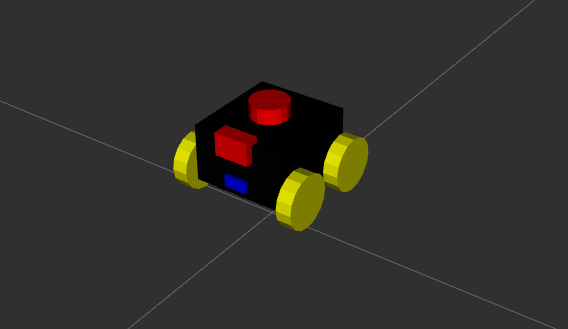
\includegraphics[scale=0.5]{obrazky-figures/robot_description.png}
	\caption{}
	\label{}
\end{figure}

\subsubsection*{Odometrie}
Druhým krokem k mapování a lokalizaci je získání aktuální pozice robota. K tomu slouží odometrie. Odometrická dala lze získat několika způsoby. Jedním z nich je změření jakou vzdálenost urazili jednotlivá kola diferenciálního robota. K tomu je však potřeba aby robot disponoval motory s enkodéry. Druhou možností je využítí imu senzoru a pomocí dat z gyroskopu a akcelerometru vypočítat aktuální pozici a natočení robota vůči počátku. Tento přístup je využit v této práci. Tuto funkcionalitu zajišťuje uzel \verb|doplnit|, který s využitím dat z imu počítá aktuální pozici a následně tyto data odesílá jako odom frame do tf topicu. Výsledná data lze opět vizualizovat v rviz, a nyní když se s robotem začně pohybovat bude tento pohyb viditelný.

\begin{figure}[h!]
	\centering
	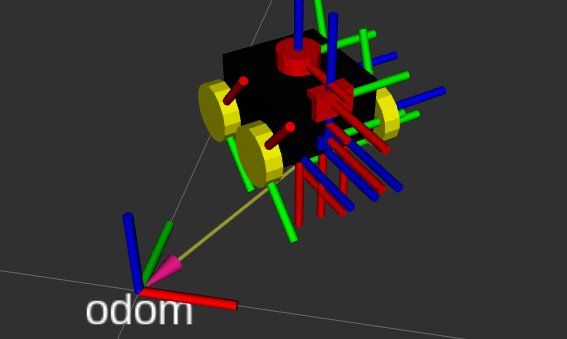
\includegraphics[scale=0.5]{obrazky-figures/odom.png}
	\caption{}
	\label{}
\end{figure}

\subsubsection*{Mapování}
Posledním krokem k úspěšnému mapování je získání dat o okolním prostředí. To zajíštuje lidar senzor umístěný na robotu. Aby bylo možné data získané z lidaru správně vizualizovat v rviz musí existovat transformace mezi lidarem a base frame robota. Pokud je lidar součástí definice modelu, postará se o tuto transformaci robot state publisher. Samotné mapování zajištuje knihovna \verb|slam-toolbox|. Ta po spuštění uzlu zpracuje data získaná z odom a scan topiců a výslednou mapu publikuje na /map topicu. Pro vizualizaci lze opět využít rviz.

\begin{figure}[h!]
	\centering
	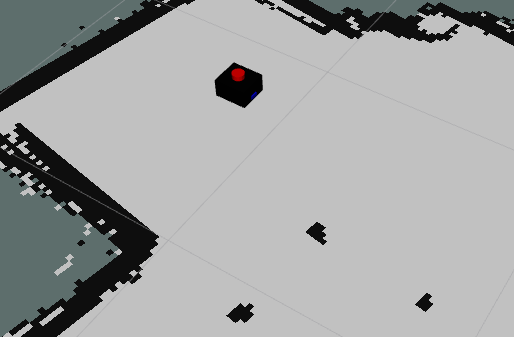
\includegraphics[scale=0.4]{obrazky-figures/slam.png}
	\caption{}
	\label{}
\end{figure}

\subsubsection*{Navigace}
Navigaci zajišťuje knihovna NAV2. Jedná se o několik spolupracujících uzlů. Základem nav2 jsou behaviorální stromy. Co se týče použití nav2 na vstupu čte odom scan a map topicy. Na výstupu pak vysílá costmapy. Mapy zobrazující co aktuálně robot vydí a ceny pro pohyb přes pozice. Pro vizualizaci lze takovou cost mapu přeložit přes mapu vytvořenou slamem. Nav2 následně poslouchá na topicu \verb|dopln| příkazy, podle kterých se následně snaží dosáhnout výsledné pozice a orientace robota. 

\begin{figure}[h!]
	\centering
	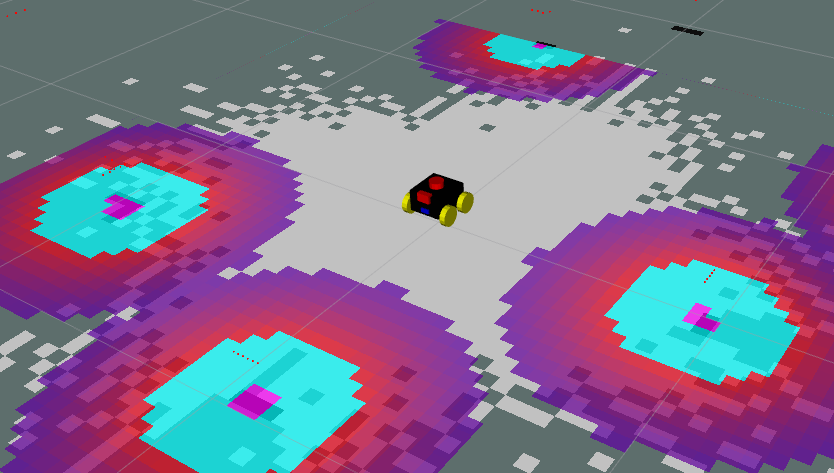
\includegraphics[scale=0.4]{obrazky-figures/nav2.png}
	\caption{}
	\label{}
\end{figure}







\section{Gazebo Simulátor}


Před tím, než lze začít využívat výhody simulátoru, je nejprve potřeba vytvořit model robota a světy ve kterých se bude pohybovat. Nativním formátem který gazebo využívá je \verb|.sdf|. V tomto formátu jsou definovány světy.

\subsection*{Definice světa}
Definice světů se skládá ze dvou základních částí. Nejprve se zpravidla definují obecné vlastnosti jako parametry simulace, fyzikální charakteristiky světa a pluginy. Druhou částí je pak samotná definice objektů, které se budou ve světě nacházet. Ty můžou být složené z jednoduchých tvarů, které lze definovat přímo v souboru. Druhou možností je vložit pomocí \verb|<mesh>| tagu složitější tvary. Poslední možností je využití oficiální fuel knihovny, která obsahuje mnoho uživateli vytvořených modelů, které lze jednoduše vložit do světa.

\subsection*{Definice modelu}
Pro definici modelu robota lze použít také SDF formát. Takto definovaný model lze vložit do světa buď přímo rámci jeho definice, nebo pomocí \verb|<include>| tagu. Druhým a z důvodu kompatibility s dalšími ROS funkcionalitami častěji používaným formátem je URDF, potažmo Xacro. 

\subsubsection*{Obecná definice}
Společné pro všechny zmíněné formáty je základní struktura složená z \verb|<link>| a \verb|<joint>| prvků. Linky reprezentují fyzické části robota jako jeho tělo či kola. Joint(kloub) pak tvoří nějaký vztah mezi linky. Jointy můžou být fixní nebo různými způsoby pohyblivé. K tomu aby model něco dělal slouží \verb|<plugin>| tagy. Ty umožnují přiřadit částem robota funkcionalitu definovanou pluginem. V gazebu existuje mnoho vestavěných pluginů jako \verb|DiffDrive| pro řízení diferenciálního pohonu nebo \verb|JointController| pro ovládání kloubů s chováním podobným servu. Naopak pro získávání informací ze simulátoru slouží \verb|<senzor>| tagy. Gazebo podporuje řadu různých senzorů. Typicky se jedná o komplexnější senzory jako lidar a hloubkové kamery. Naopak jednodušší senzory typu ultrazvukový, či sledování čáry nejsou v repertoáru. V implementaci bylo tedy potřeba využít těch podporovaných k simulaci těch nepodporovaných. Ultrazvukový senzor vzdálenosti je tedy ve výsledném modelu nahrazen lidar senzorem s omezeným úhlem a počtem paprsků. Modul pro sledování čáry je pak realizován pomocí kamer s rozlišením jeden pixel který je v kódu převeden na grayscale hodnotu a pomocí treasholdingu rozhodnut výsledek.

\subsubsection*{Xacro Specifika}
Jak už bylo řečeno, výsledný model je definován ve formátu Xacro. Pro delší definice je tento formát velmi vhodný, protože použití čistého URDF, vede na dlouhý, repetitivní a na chyby náchylný XML kód. Jednou z nejčastěji opakovaných sekcí v URDF kódu je téměř totožná definice fyzikálních vlastností \verb|<link>| elementu. Obsahuje určení váhy, setrvačnosti, a tvaru pro vizuální, kolizní část robota. S použitím XACRO lze tuto část definovat jako makro s několika parametry a následně jedním řádkem vkládat do složitějších definic, kde by tato část jen překážela. Díky matematice se jako součást makra vypočítají i matice setrvačnosti, kterou je jinak potřeba počítat ručně. Podobné makro je pak také definováno pro <joint> elementy. Tyto základní komponenty se následně využívají v rámci definice senzorů. Hlavní soubor se díky této struktuře stává krátkým a přehledným, odkud lze jednoduše a rychle nalézt konkrétní komponenty robota a provádět na nich změny.

Výsledný Xacro soubor je před použitím v simulátoru nejprve potřeba přeložit do URDF formátu. K tomu slouží příkaz \verb|xacro [in.xacro] > [out.urdf]|. Modely definované v URDF se do světa \uv{spawnují} a to až po spuštění simulace. Slouží k tomu gazebo service jménem \verb|/world/name/create| a příkaz \verb|ign service|. 

\subsubsection*{ROS Gazebo Bridge}
Komunikaci mezi Gazebo simulátorem a zbytkem ROS2 systému zajišťuje oficiální nástroj \verb|ros_gz_bridge|. Tento most na jedné straně interaguje s gazebo reprezentací topiců a servisů. Na druhé straně se pak tváří jako ROS2 uzel. Spouští se pomocí příkazu:
\begin{verbatim}
	ros2 run ros_gz_bridge parameter_bridge /topic_name@gazebo_msg_type@ignition_msg_type
\end{verbatim}
Pro efektivnější použití lze předat bridge uzlu config soubor s definicí více topiců které budou přemostěny.
\begin{verbatim}
- ros_topic_name: "ros_chatter"
  gz_topic_name: "gz_chatter"
  ros_type_name: "std_msgs/msg/String"
  gz_type_name: "gz.msgs.StringMsg"
  direction: IGN_TO_ROS  # BIDIRECTIONAL or ROS_TO_IGN
\end{verbatim}

\chapter{Závěr}
%cca strana

%===============================================================================

% Pro kompilaci po částech (viz projekt.tex) nutno odkomentovat
%\end{document}
